\documentclass{article}\usepackage[]{graphicx}\usepackage[]{color}
%% maxwidth is the original width if it is less than linewidth
%% otherwise use linewidth (to make sure the graphics do not exceed the margin)
\makeatletter
\def\maxwidth{ %
  \ifdim\Gin@nat@width>\linewidth
    \linewidth
  \else
    \Gin@nat@width
  \fi
}
\makeatother

\definecolor{fgcolor}{rgb}{0.345, 0.345, 0.345}
\newcommand{\hlnum}[1]{\textcolor[rgb]{0.686,0.059,0.569}{#1}}%
\newcommand{\hlstr}[1]{\textcolor[rgb]{0.192,0.494,0.8}{#1}}%
\newcommand{\hlcom}[1]{\textcolor[rgb]{0.678,0.584,0.686}{\textit{#1}}}%
\newcommand{\hlopt}[1]{\textcolor[rgb]{0,0,0}{#1}}%
\newcommand{\hlstd}[1]{\textcolor[rgb]{0.345,0.345,0.345}{#1}}%
\newcommand{\hlkwa}[1]{\textcolor[rgb]{0.161,0.373,0.58}{\textbf{#1}}}%
\newcommand{\hlkwb}[1]{\textcolor[rgb]{0.69,0.353,0.396}{#1}}%
\newcommand{\hlkwc}[1]{\textcolor[rgb]{0.333,0.667,0.333}{#1}}%
\newcommand{\hlkwd}[1]{\textcolor[rgb]{0.737,0.353,0.396}{\textbf{#1}}}%
\let\hlipl\hlkwb

\usepackage{framed}
\makeatletter
\newenvironment{kframe}{%
 \def\at@end@of@kframe{}%
 \ifinner\ifhmode%
  \def\at@end@of@kframe{\end{minipage}}%
  \begin{minipage}{\columnwidth}%
 \fi\fi%
 \def\FrameCommand##1{\hskip\@totalleftmargin \hskip-\fboxsep
 \colorbox{shadecolor}{##1}\hskip-\fboxsep
     % There is no \\@totalrightmargin, so:
     \hskip-\linewidth \hskip-\@totalleftmargin \hskip\columnwidth}%
 \MakeFramed {\advance\hsize-\width
   \@totalleftmargin\z@ \linewidth\hsize
   \@setminipage}}%
 {\par\unskip\endMakeFramed%
 \at@end@of@kframe}
\makeatother

\definecolor{shadecolor}{rgb}{.97, .97, .97}
\definecolor{messagecolor}{rgb}{0, 0, 0}
\definecolor{warningcolor}{rgb}{1, 0, 1}
\definecolor{errorcolor}{rgb}{1, 0, 0}
\newenvironment{knitrout}{}{} % an empty environment to be redefined in TeX

\usepackage{alltt}

\usepackage{rotating}
\usepackage{graphics}
\usepackage{latexsym}
\usepackage{color}
\usepackage{listings} % allows for importing code scripts into the tex file
\usepackage{wrapfig} % allows wrapping text around a figure
\usepackage{lipsum} % provides Latin text to fill up a page in this illustration (do not need it otherwise!)

% Approximately 1 inch borders all around
\setlength\topmargin{-.56in}
\setlength\evensidemargin{0in}
\setlength\oddsidemargin{0in}
\setlength\textwidth{6.49in}
\setlength\textheight{8.6in}

% Options for code listing; from Patrick DeJesus, October 2016
\definecolor{codegreen}{rgb}{0,0.6,0}
\definecolor{codegray}{rgb}{0.5,0.5,0.5}
\definecolor{codepurple}{rgb}{0.58,0,0.82}
\definecolor{backcolour}{rgb}{0.95,0.95,0.92}
\lstdefinestyle{mystyle}{
	backgroundcolor=\color{backcolour},   commentstyle=\color{codegreen},
	keywordstyle=\color{magenta},
	numberstyle=\tiny\color{codegray},
	stringstyle=\color{codepurple},
	basicstyle=\footnotesize,
	breakatwhitespace=false,         
	breaklines=true,                 
	captionpos=b,                    
	keepspaces=true,                 
	numbers=left,                    
	numbersep=5pt,                  
	showspaces=false,                
	showstringspaces=false,
	showtabs=false,                  
	tabsize=2
}

%"mystyle" code listing set
\lstset{style=mystyle}
%\lstset{inputpath=appendix/}


\title{Predictions on Whether a Tumor has Penetrated the Prostatic Capsule} 
\author{Kelso Quan}
\IfFileExists{upquote.sty}{\usepackage{upquote}}{}
\begin{document} 

\maketitle
\begin{center}
\Large{Abstract}
\end{center}

Prostate cancer is one of the most common cancers among men. Luckily, prostate cancer is treatable when detected early enough. The Ohio State University Comprehensive Cancer Center wants to know if baseline exam measurements can predict whether a tumor has penetrated the prostatic capsule indicating there is indeed a tumor present. The Prostatic Specific Antigen value (PSA), results of digital exam (dpros), and total Gleason score has the ability of predicting whether a patient has a tumor penetrating the prostatic capsule. A patient that has a right unilobar nodule has up to 4.73 times the odds of having their prostatic capsule penetrated by a tumor compared to patients that has no presence of a nodule. For every increase of total Gleason score, there is an additional increase of 2.71 odds likely of having a tumor puncture the prostatic capsule. With every 1 mg/ml increase of PSA, there will be an increase of 3 \% odds in having a tumor penetrate the capsule. For one of the predictions, a patient that has bilobar nodule with PSA of 25 and a total Gleason score of 9 has 2.58 times more likely odds of having a tumor protruding from their prostatic capsule. In the end, this model does not have any interaction terms even though they were considered within the scope of the analysis. 

\section{Introduction}
\qquad Since prostate cancer is one of the most common cancer among men, a study was conducted at the Ohio State University Comprehensive Cancer Center tried to determine if a tumor has penetrated the prostatic capsule. This is good news for a majority of men. Prostate cancer which occurs in about 1 out of 7 men, but only 1 in 39 men will die due to this cancer according to webmd. Several factors contribute to cancer tumors penetrating the prostatic capsule which include: age of subject, race, results of digital exam, detection of capsular involvement, Prostatic Specific Antigen value, and total Gleason score. It appears that the Prostatic Specific Antigen value (PSA), results of digital exam, and total Gleason score is able to predict whether a patient has a tumor penetrating the prostatic capsule. 


\section{Methods}
\qquad There was a cancer study on 380 male patients of either white or black race. Patients 1162, 1186, 1392 were excluded because those patients had at least one ``na" value listed. For those who do not know about prostate cancer, many of the variables will seem unfamiliar. PSA is a measure of protein produced by prostate gland cells and is measured in $mg/mL$. Elevated levels of PSA may suggest prostate cancer and is used as a screening test. The total Gleason score is a scale from 1 to 10 measuring the abnormality of cells. Larger values of Gleason score suggest a higher risk of cancer. Race has two factors, whether the patient is black or white. The variable capsule indicates whether the tumor penetrated the prostatic capsule. dpros are the results of the digital rectal exam which can have no nodule, unilobar (left and right) nodule, bilobar nodule. dcaps is the detection of capsular involvement. There was 153 of the 380 subjects who had a cancer that penetrated the capsule. 

\qquad This analysis will not have any transformations, but will consider interaction terms. 
The analysis will be conducted using R/RStudio. 

\section{Results}
\subsection{Exploratory Data Analysis}
\begin{figure}
\caption{Boxplot of PSA/Gleason vs Capsule Penetration}
\label{boxplot}
\begin{knitrout}
\definecolor{shadecolor}{rgb}{0.969, 0.969, 0.969}\color{fgcolor}
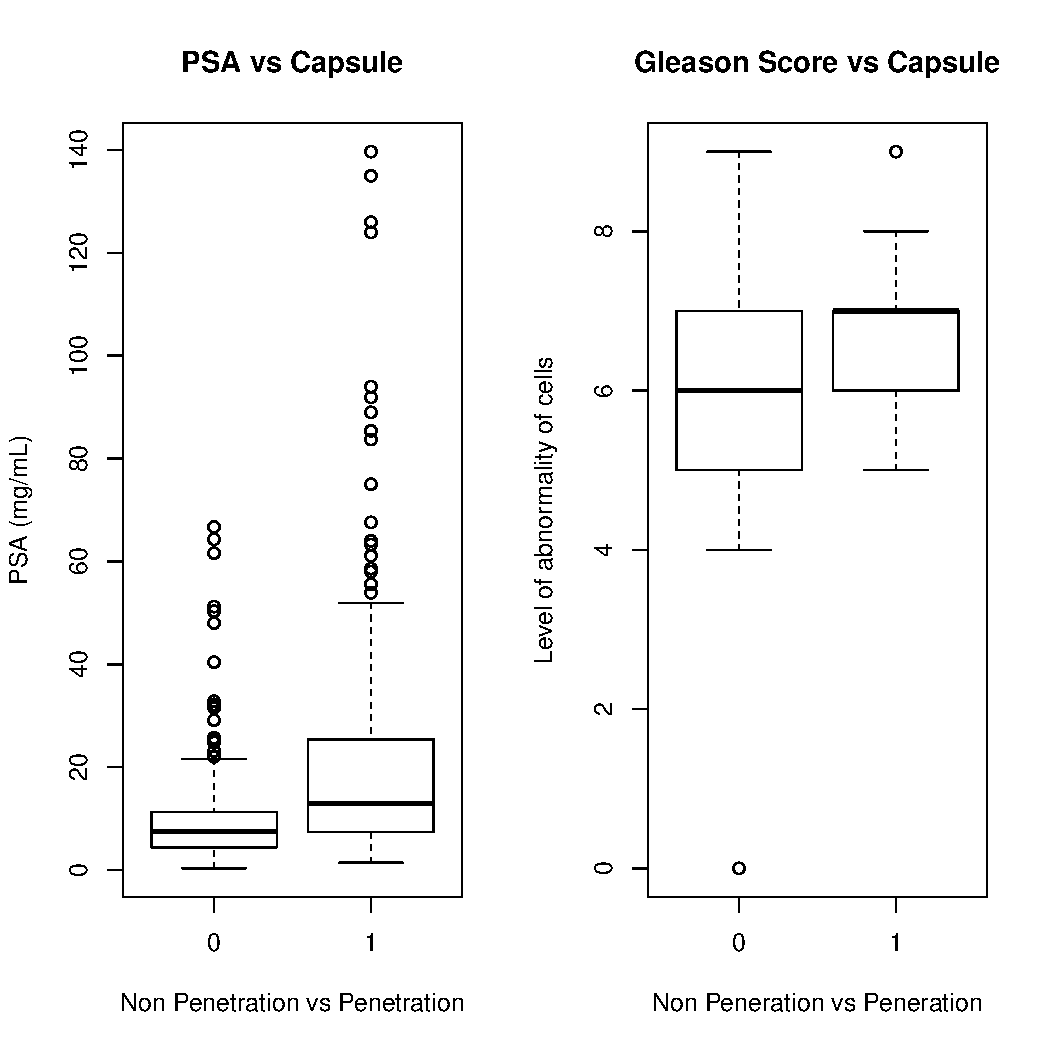
\includegraphics[width=\maxwidth,height=0.4\textheight]{figure/Boxplot-1} 

\end{knitrout}
\end{figure}
\qquad In figure \ref{boxplot}, it shows two things, the amount of PSA when the capsule is penetrated and the distribution of having the capsule penetrated given the level of abnormality in the cells. Both boxplots include patients without a tumor penetrating the capsule. This did show some interesting results. PSA is higher when the capsule is penetrated and the Gleason score is generally higher when there is penetration. These two graphs shows that the doctors and scientists at Ohio State were onto something. In figure \ref{diagnostics} shows that there are not any serious violations of homoscedasticity pictured in the Standardized Pearson residual plot. Also, there are very few observations with this model that went beyond three standard deviations. There is a couple of influential points coming from the Cook's distance vs leverage plot that should be discussed. But after examining the possible outliers, these outliers do not significantly impact the model. By applying the HL test, the p-value is 0.246 which means fail to reject the chosen model. 
\begin{figure}
\caption{Diagnostic Plots of the model: Capsule = PSA + Gleason + Dpros}
\label{diagnostics}
\begin{knitrout}
\definecolor{shadecolor}{rgb}{0.969, 0.969, 0.969}\color{fgcolor}
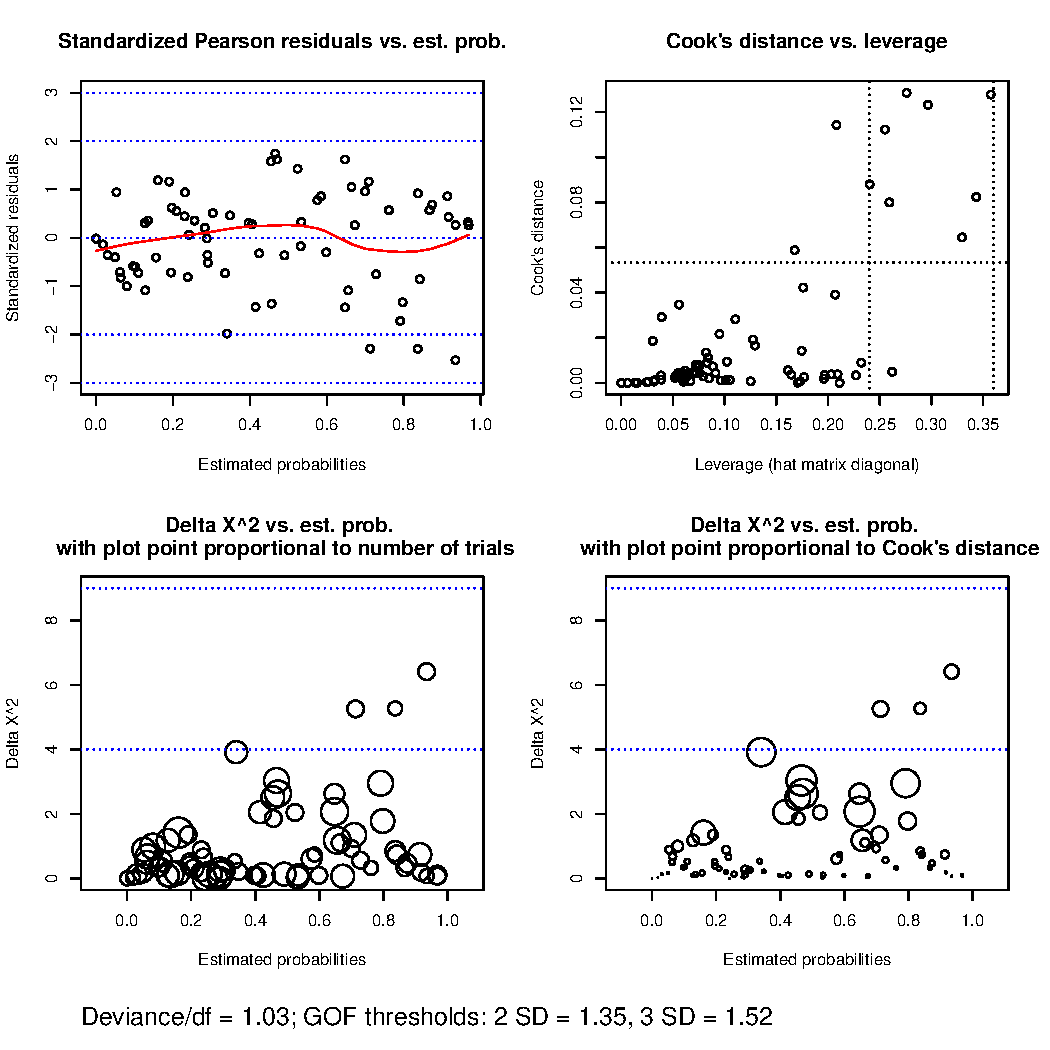
\includegraphics[width=\maxwidth]{figure/Diagnostics_Charts-1} 

\end{knitrout}
\end{figure}

\subsection{Model Fitting/Inferences}
\qquad By using the stepAIC on all possible models containing interaction terms, the model with the least of amount of penalties still had non significant terms. Manually, the terms that were not significant by p-values were dropped one-by-one out of the model. Eventually, the model contained three predictor variables that were not highly correlated with each other shown in figure \ref{corrplot} in the appendix. just at a glance, the correlation plot also shows that the total Gleason score is moderately correlated to a tumor penetration of the prostatic capsule.

\qquad Interpreting an odds ratio is is not too difficult. Any odds ratio at 1 does not influence the response. Odds ratios that are between 0 and 1 are (1 - odds ratio) * 100\% less odds of having the capsule penetrated by a tumor. But with an odds ratio greater than 1 and less than 2, then the patient has (odds ratio - 1) * 100\% more odds of having the capsule penetrated by a tumor. For example, PSA has a coefficient of .03 and has 1.03 odds ratio which means that with 1 mg/mL increase in PSA while all other variables are held constant means a patient has $3\%$ increase in odds of having the capsule penetrated by a tumor for every 1 mg/mL increase in PSA according to table \ref{odds}. With an odds ratio greater than 2, that odds ratio becomes a factor increase. The odds ratio of total Gleason score is 2.71 which means the patient's odds of having their capsule penetrated by a tumor is increased by a factor 2.71 times for every 1 additional Gleason score added. The rest of the odds ratio can be interpreted in a similar manner, but take caution when interpreting the intercept or any of the dpros predictors. The intercept should be seen as no penetration or dpros1, whereas dpros2 and dpros 3 are directional. In addition, there are confidence intervals associated with their respective odds ratio.

\begin{table}[ht]
\centering
\caption{Odds Ratio with 95\% CI on Odds Ratio}
\label{odds}
\begin{tabular}{|l|ccccc|}
  \hline
 & Coefficient & Odds Ratio & SE & p-value & 95\% CI on OR \\ 
  \hline
intercept & -8.14 & 0.00 & 1.06 & 0.0000 & ( 0.00 , 0.00 ) \\ 
  dpros2 & 0.77 & 2.17 & 0.36 & 0.0300 & ( 1.09 , 4.43 ) \\ 
  dpros3 & 1.55 & 4.73 & 0.37 & 0.0000 & ( 2.32 , 10.00 ) \\ 
  dpros4 & 1.43 & 4.18 & 0.45 & 0.0015 & ( 1.75 , 10.20 ) \\ 
  psa & 0.03 & 1.03 & 0.01 & 0.0036 & ( 1.01 , 1.05 ) \\ 
  gleason & 0.99 & 2.71 & 0.16 & 0.0000 & ( 2.00 , 3.76 ) \\ 
   \hline
\end{tabular}
\end{table}
With this model, a patient's odds of a tumor penetrating their prostatic capsule can be determined. Based on table \ref{prediction}, there are several values that were simulated to see a patient's odds of whether a tumor has penetrated their prostatic capsule. For an example, take a patient that has a unilobar nodule on his right side, with PSA of 14.1 and a total Gleason score of 7, then that patient has 98\% more likely odds of having a tumor protruding into their capsule. 
\begin{table}
\begin{center}
\caption{Predictions on Simulated values}
\label{prediction}
\begin{tabular}{c|c|c|c}
Odds Ratio & dpros & PSA & Gleason \\
\hline
1.98 & unilobar nodule (right) & 14.1 & 7 \\
2.23 & unilobar nodule (left) & 30 & 8 \\
2.58 & bilobar nodule & 25 & 9 \\
1.31 & unilobar module (left) & 15.25 & 6\\
\end{tabular}
\end{center}
\end{table}
\section{Conclusions}
\quad 
The analysis has shown that total Gleason score, Prostatic Specific Antigen value, and results of a digital rectal exam are the best variables that can predict the probability a man will have a tumor penetrating the prostatic capsule. In the table \ref{odds}, showed that the results from the digital rectal exam had the most influence on whether a male patient had a tumor protruding through the prostatic capsule. A patient that had a right unilobar nodule had up to 4.73 times the odds of having their capsule penetrated compared to patients that had no presence of a nodule. For every 1 level of total Gleason score increase, there is increase of 2.71 odds likely of having a tumor puncture the prostatic capsule. With every 1 mg/ml increase of PSA, there will be an increase about 3\% odds in having a tumor penetrate the capsule.
Refer to table \ref{prediction} to see some simulated patients and their odds of having a tumor penetrate the prostate capsule. A patient that has a unilobar nodule on his left side, with PSA of 30 and a total Gleason score of 8 means that patient has 2.23 more likely odds of having a tumor protruding into their capsule.

There were several limitations of this study. Age did not play a major factor in the model since the study focused on older men with the youngest man being 47 in the study. If the study included younger men from the ages of 18-35, one can speculate that age will play a huge factor in predicting whether those young men had a tumor penetrate their prostate capsule. 
In addition, a table showing race would say that only 36 patients were black. That number may or may not be enough to figure out whether this model is works well for black patients, but a simple power calculation would suffice. Furthermore, the results of this study should only apply to those older black or white gentlemen due to the scope of the study.
An important question for doctors and scientists is whether prostate cancer can be predicted before a cancerous tumor has penetrated the prostatic capsule. If prostate cancer can be detected even before it has punctured the capsule, then the rate of survival can be raised even higher than the current rate. 
\newpage
\noindent \Large{{\bf Appendix A: Auxiliary Graphics and Tables}}
\begin{figure}
\caption{Correlation plot among Covariates and Response}
\label{corrplot}
\begin{knitrout}
\definecolor{shadecolor}{rgb}{0.969, 0.969, 0.969}\color{fgcolor}\begin{kframe}


{\ttfamily\noindent\itshape\color{messagecolor}{\#\# corrplot 0.84 loaded}}\end{kframe}
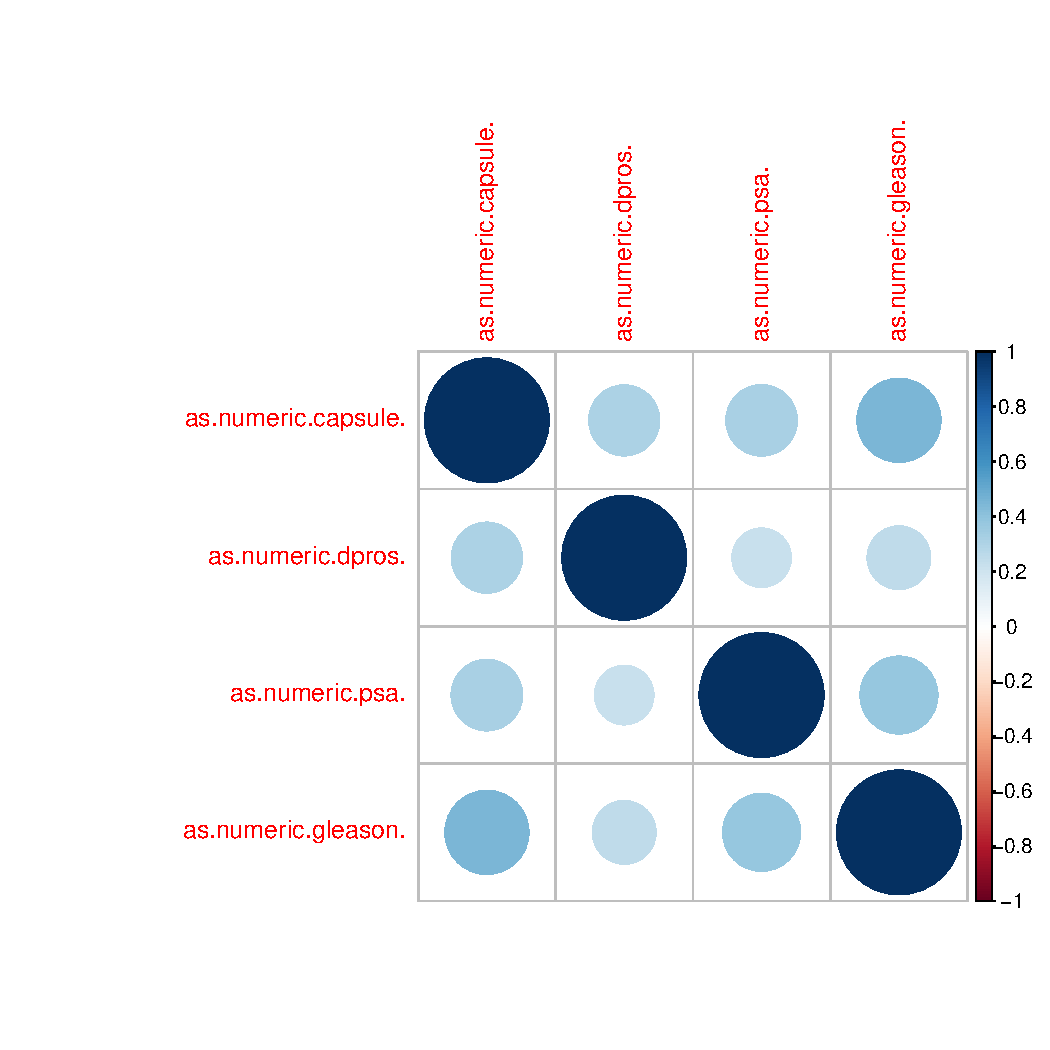
\includegraphics[width=0.5\linewidth,height=0.5\textheight]{figure/Corrplot-1} 

\end{knitrout}
\end{figure}

\begin{table}
\begin{center}
\caption{Race vs Tumor penetration of prostatic capsule}
\label{race}
\begin{tabular}{c|c|c}
 & White & Black \\ \hline
No Penetration & 204 & 22\\
Penetration & 137 & 14 \\
\end{tabular}
\end{center}
\end{table}

\begin{table}
\begin{center}
\caption{Total Gleason Score vs Tumor penetration of prostatic capsule}
\label{gleason}
\begin{tabular}{c|c|c|c|c|c|c|c}
   &0 &  4 &  5  & 6 &  7 &  8  & 9 \\ \hline
      No Penetration &  2 &  1 & 61 & 100 & 55 &  6  & 1 \\
      Penetration &  0  & 0 &  6 & 38 & 72 & 23 & 12 \\
\end{tabular}
\end{center}
\end{table}


\begin{table}
\begin{center}
\caption{Digital Rectal Exam Results vs Tumor penetration of prostatic capsule}
\label{race}
\begin{tabular}{c|c|c|c|c}
 & No Nodule & Left Nodule & Right Nodule  & Bilobar Nodule \\ \hline
      No Penetration & 80 & 83 & 45 & 18 \\
      Penetration & 19 & 48 & 50 & 34\\
\end{tabular}
\end{center}
\end{table}

\begin{table}
\begin{center}
\caption{Detection of capsular involvement vs Tumor penetration of prostatic capsule}
\label{dcaps}
\begin{tabular}{c|c|c}
 & No & Yes \\ \hline
No Penetration & 216 & 10\\
Penetration & 121 & 30 \\
\end{tabular}
\end{center}
\end{table}
\newpage
\noindent \Large{{\bf Appendix B: R Code}}


\lstinputlisting[language=R, caption = Prostate Cancer]{ProDAR.R}
\end{document}
